\chapter{Présentation du projet}


\section{Introduction}

.\renewcommand{\abstractnamefont}{\normalfont\Large\bfseries}
%\renewcommand{\abstracttextfont}{\normalfont\Huge}

\begin{abstract}
\hskip7mm

\begin{spacing}{1.3}

Lorem ipsum dolor sit amet, consectetur adipiscing elit. Sed non risus. Suspendisse lectus tortor, dignissim sit amet, adipiscing nec, ultricies sed, dolor. Cras elementum ultrices diam. Maecenas ligula massa, varius a, semper congue, euismod non, mi. Proin porttitor, orci nec nonummy molestie, enim est eleifend mi, non fermentum diam nisl sit amet erat. Duis semper. Duis arcu massa, scelerisque vitae, consequat in, pretium a, enim. Pellentesque congue. Ut in risus volutpat libero pharetra tempor. Cras vestibulum bibendum augue. Praesent egestas leo in pede. Praesent blandit odio eu enim. Pellentesque sed dui ut augue blandit sodales. Vestibulum ante ipsum primis in faucibus orci luctus et ultrices posuere cubilia Curae; Aliquam nibh. Mauris ac mauris sed pede pellentesque fermentum. Maecenas adipiscing ante non diam sodales hendrerit. Ut velit mauris, egestas sed, gravida nec, ornare ut, mi. Aenean ut orci vel massa suscipit pulvinar. Nulla sollicitudin. Fusce varius, ligula non tempus aliquam, nunc turpis ullamcorper nibh, in tempus sapien eros vitae ligula. Pellentesque rhoncus nunc et augue. Integer id felis. Curabitur aliquet pellentesque diam. Integer quis metus vitae elit lobortis egestas. Lorem ipsum dolor sit amet, consectetuer adipiscing elit. Morbi vel erat non mauris convallis vehicula. Nulla et sapien. Integer tortor tellus, aliquam faucibus, convallis id, congue eu, quam. Mauris ullamcorper felis vitae erat. Proin feugiat, augue non elementum posuere, metus purus iaculis lectus, et tristique ligula justo vitae magna. Aliquam convallis sollicitudin purus. Praesent aliquam, enim at fermentum mollis, ligula massa adipiscing nisl, ac euismod nibh nisl eu lectus. Fusce vulputate sem at sapien. Vivamus leo. Aliquam euismod libero eu enim. Nulla nec felis sed leo placerat imperdiet. Aenean suscipit nulla in justo. Suspendisse cursus rutrum augue. Nulla tincidunt tincidunt mi. Curabitur iaculis, lorem vel rhoncus faucibus, felis magna fermentum augue, et ultricies lacus lorem varius purus. Curabitur eu amet.

\end{spacing}
\end{abstract}
\\
Pour utiliser le programme, il faut donner en argument le fichier pcap a analyser (pas encore possible de choisir le protocole).

\section{Présentation du fichier Pcap}

La première chose a effectué lors de l'ouverture du fichier pcap, est l'extraction du "Global Header" du fichier.
Il contient plusieurs informations essentielles à la compréhension du fichier, notamment l'encodage des informations binaire.
Si Les informations sont codés selon la norme "Big-Endian" dans ce cas, on accepte d'ouvrir le fichier, sinon on le rejette.
Pour la norme Little-Endian il faut inverser chaque octet.

La figure ci-dessous montre comment est composé le fichier pcap.
\begin{figure}[!h]
    \begin{center}
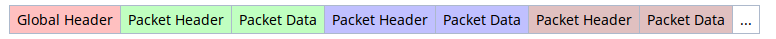
\includegraphics[width=15cm]{./globalHeader.png}
    \end{center}
\end{figure}

Dans ce fichier, chaque paquet est composé de deux choses:
\begin{itemize}
    \item Un Header Pcap;
    \item Un Packet Data.
\end{itemize}       
Le header donne les informations de base du paquet.
Les données correspondent au paquet réseau. 
Pour commencer, j'ai créé un objet pour rassembler les informations contenu dans le pcap header, et un second objet qui correspond au donnée.
Ensuite dans chaque objet, il existe un attribut qui a pour type un tableau d'octets et qui contient les informations du fichier pcap.
Ensuite une methode permet d'extraire les octets qui nous intéresse pour les analyser.
Par exemple, on peut utliser cette méthode pour extraire les 4 premiers octets et vérifier que ces octets sont égaux à "d4c3b2a1".


\section{Les différents objets du projet}

Les réseaux sont construit autour du modèle OSI, lui-même divisé en 7 couches.
Pour ce projet, j'ai créé un objet par couche. Les informations contenu dans l'objet "Header Pcap" contiennent les données sur la première couche de ce modèle.
Sur chaque couche, j'ai créé plusieurs méthodes permettant de récuperer les informations intéressante.
Puis ensuite, j'ai créé plusieurs objets par protocoles. Certains protocoles comme TCP et UDP héritent de la classe "Couche4".

Le premier objet est le pcapheader. Il contient:
\begin{itemize}
    \item Le temps en sec;
    \item Le temps original du paquet;
    \item La taille du paquet;
    \item La teille effective du paquet ;
    \item Les donnée du paquet.
\end{itemize}   

Ensuite on envoie les donnée du paquet a la couche 2 du modèle OSI.
Une méthode de l'objet determine les informations du paquet, si un protocole est detecté, on crée un objet pour ce protocole et on envoie les inforamtions du paquet à l'objet.
Sur chaque couche du modèle OSI, on a une encapsulation des paquets. Par exemple les informations de la couche 3 sont contenus dans la charge utile de la couche2.
Sur chaque analyse de paquet, lorsque l'on détecte une couche en plus, on crée un objet correspondant à cette couche.

On descend au fur et à mesure dans les couche. Si à un moment, on trouve un protocole, dans ce cas on arrête de monter dans les couches et on affcihe les dernières informations du paquet.

Pour chaque paquet, on affiche les informations couche par couche, en terminant par le protocole.
Chaque objet a sa méhode "Informations" qui permet d'afficher les informations pertinante de la couche en cours d'analyse.
\subsection{couche 2}
La couche 2 est constituée:
\begin{itemize}
    \item Une adresse MAC Source;
    \item Une adresse MAC Destination;
    \item Un éventuel protocole;
    \item Une charge utile.
\end{itemize}      
    \subsubsection{ARP}
L'objet ARP étend la couche2 est constitué:
\begin{itemize}
    \item du hardware type;
    \item du prototype type;
    \item du type de requête (Request ou Reply);
    \item de l'IP Source;
    \item de l'IP Destination.
\end{itemize}      
Si les informations du header de la couche 2 n'indique pas que le protocole suivant est ARP ou IP. On arrête l'analyse.

\subsection{couche 3}
La couche 3 est constituée de toute les informations concernant IP:
\begin{itemize}
    \item Version;
    \item taille;
    \item ttl;
    \item protocole suivant;
    \item IP Source;
    \item IP Destination;
    \item une charge utile.
\end{itemize}      
Si le protocole de couche 3 est différents d'IPv4, on abandonne l'analyse.
Si on détecte ICMP, TCP, UDP, on continue l'analyse et on créé l'objet correspondant.

\subsection{couche 4}
La couche 4 est constituée:
\begin{itemize}
    \item Port Source;
    \item Port Destination;
    \item protocole;
    \item charge utile.
\end{itemize}      
En fonction du protocole, on créé les objets suivants:
    \subsubsection{ICMP}
L'objet ICMP est constitué:
\begin{itemize}
    \item type;
    \item code;
    \item checksum;
\end{itemize}      
En fonction du code, on determine la requete ICMP qui est effectué (Request ou reply ou ttl exceed, ou destination unreacheable).

    \subsubsection{TCP}
L'objet TCP étends l'objet Couche4, il est constitué:
\begin{itemize}
    \item port Source;
    \item port Destination;
    \item taille;
    \item flags;
    \item charge utile;
\end{itemize}      
En fonction du flag on peut determiner à quel niveau du "handshake TCP" on est : SYN, SYN-ACK, ACK, Fin, Fin-ACK.

    \subsubsection{UDP}
L'objet UDP étends l'objet Couche 4, il est constitué:
\begin{itemize}
    \item Port Source;
    \item Port Destination;
    \item taille
\end{itemize}   


%%inclusion d'une mage dans le document
%\begin{figure}[!h]
%\begin{center}
%%taille de l'image en largeur
%%remplacer "width" par "height" pour régler la hauteur
%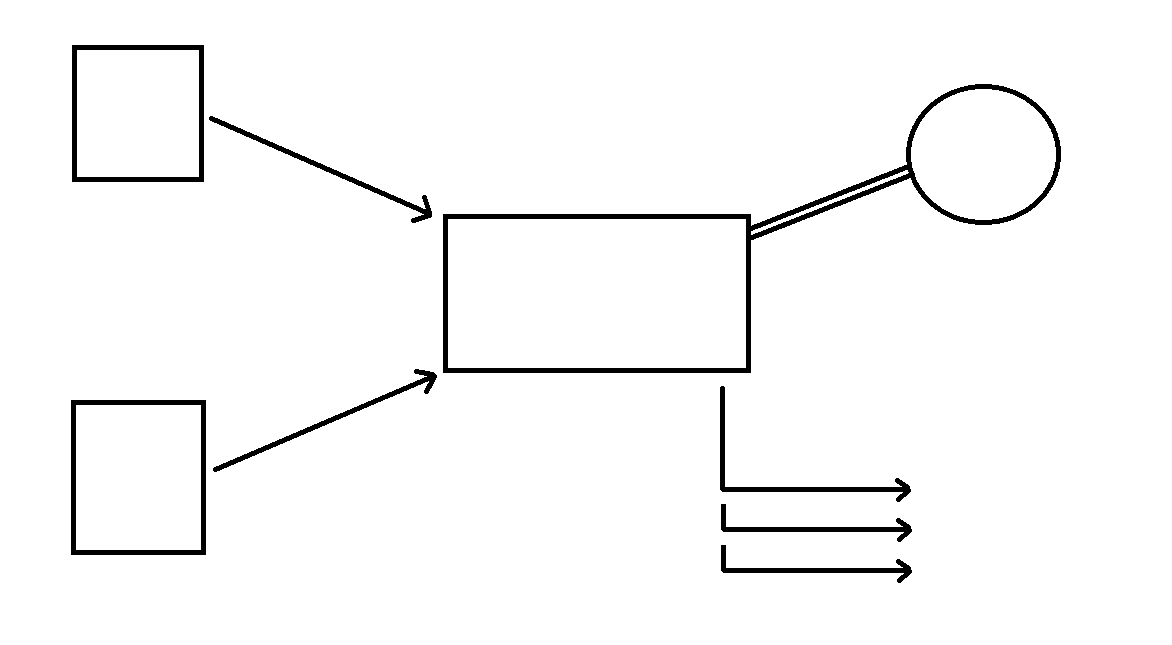
\includegraphics[width=15cm]{presentation/schema}
%\end{center}
%%légende de l'image
%\caption{Schéma descriptif}
%\end{figure}
%
%%Contenu de la note précédemment marquée avec \footnotemark
%\footnotetext{Note bas de page "intro"}
%
%Bla
%%retour à la ligne (alinea)
%
%Bla\\
%%saut de paragraphe
%
%Bla
%
%\newpage
%
%\section{Problématique soulevée}
%
%Bla
%
%\begin{center}
%Problématique du sujet
%\end{center}
%
%\section{Hypothèse de solution}
%
%%Quoi :
%Bla\\
%
%Voici une liste :
%\begin{itemize}
%\item item 1;
%\item item 2;
%\item item 3;
%\item item 4.
%\end{itemize}
%
%Bla\\
%
%%Comment :
%Bla
%
%Bla\footnotemark\\
%
%%Detail :
%Bla(cf. ref. \cite{cite6}).
%%citation référencé dans le document "bibliographie.bib" inclus à la fin du document
%
%\footnotetext{Note bas de page "bla"}
